

%%================================================= PAGE SETUP==============================================
    \renewcommand{\thesubsection}{\Alph{subsection}}                  %% Removes section number from subsection appendix

    \newcommand{\fakesection}[1]{%                          %% Creates a fake section for the TOC
      \par\refstepcounter{section}                               %% Increase section counter
      \sectionmark{#1}                                           %% Add section mark (header)
      \addcontentsline{toc}{section}{#1}}                         %% Add section to ToC

    \newcommand{\fakesubsection}[1]{%                                       %% Creates a fake subsection for the TOC
      \par\refstepcounter{subsection}                                         %% Increase section counter
      \sectionmark{#1}                                                           %% Add section mark (header)
      \addcontentsline{toc}{subsection}{\protect\numberline{\thesubsection}#1}}  %% Add subsection to ToC

    \titleformat{\subsection}                               %% Centering of the Appendix Titles
      {\large\bfseries\centering}
      {\thesection}{}{}
%%================================================END PAGE SETUP============================================



\fakesection{Appendices}                               %% Adds section to TOC but not the page


%%----------------Appendix A
\fakesubsection{\SI[per-mode=symbol]{0.35}{\cubic\meter\per\second} flow rate models} %% Adds subsection to TOC but not the page
\subsection*{Appendix A}\label{appendixA}                        %% Adds subsection to page but not the TOC

\renewcommand\thefigure{A.\arabic{figure}}                          %% Begins numbering the appendix figures with A
\setcounter{figure}{0}                                              %% Restarts the figure counter

\centering
\begin{figure}[h!]                                                   	%% 00.35 Flow rate
	\begin{tabular}{ l  c }
		
		& 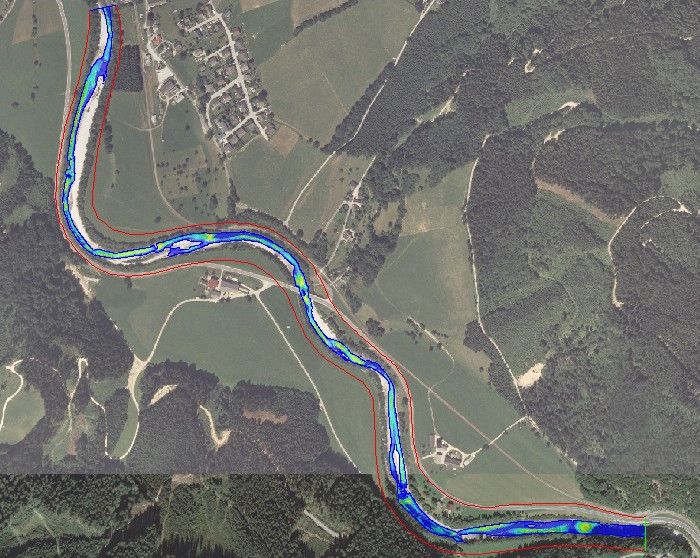
\includegraphics[width=0.56\textwidth,valign=t]{images/0_0035}\\
		& 0+ age class\\
		\multirow{4}{*}{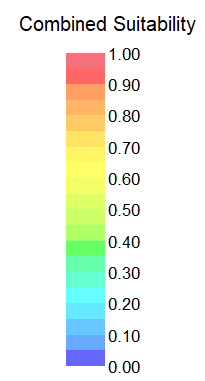
\includegraphics[width=0.3\textwidth,valign=t]{images/suitability_index}}& 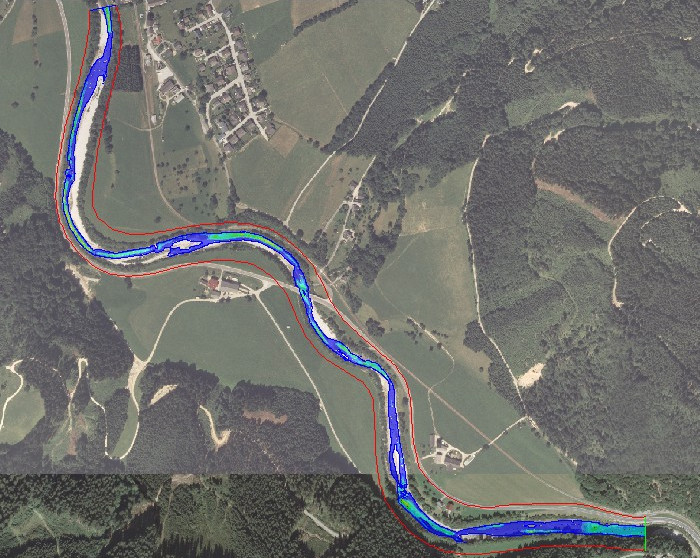
\includegraphics[width=0.56\textwidth,valign=t]{images/1_0035}\\
		& 1+ age class\\
		& 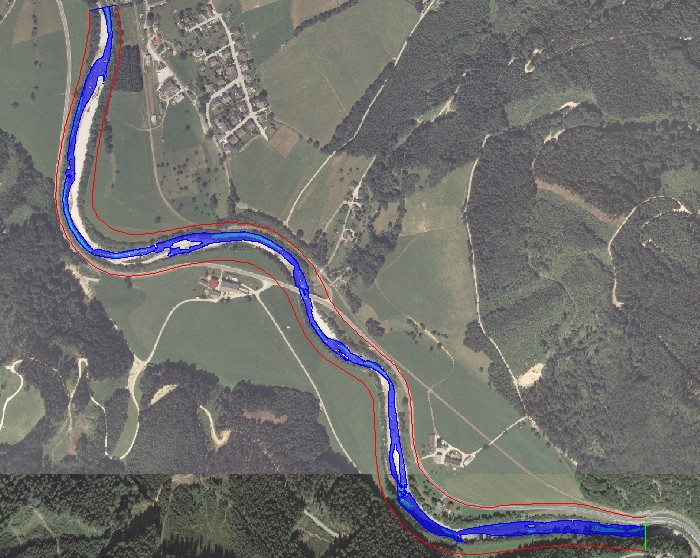
\includegraphics[width=0.56\textwidth,valign=t]{images/2_0035}\\
		& 2+ age class
		
	\end{tabular}
	\label{fig:0035}
	
	\caption{River2d models of the Ybbs river at \SI[per-mode=symbol]{0.35}{\cubic\meter\per\second}.}   %% figure Caption
	
\end{figure}


\newpage                                                                %% End page


%%----------------Appendix B
\fakesubsection{\SI[per-mode=symbol]{2.16}{\cubic\meter\per\second} flow rate models} %% Adds subsection to TOC but not the page
\subsection*{Appendix B}\label{appendixB}                        %% Adds subsection to page but not the TOC

\renewcommand\thefigure{A.\arabic{figure}}                          %% Begins numbering the appendix figures with A
\setcounter{figure}{0}                                              %% Restarts the figure counter

\centering
\begin{figure}[h!]                                                   	%% 00.35 Flow rate
	\begin{tabular}{ l  c }
		
		& 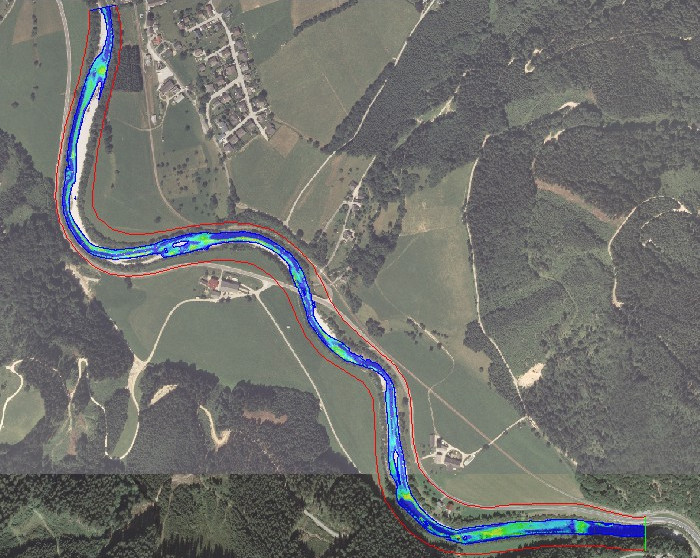
\includegraphics[width=0.56\textwidth,valign=t]{images/0_0216}\\
		& 0+ age class\\
		\multirow{4}{*}{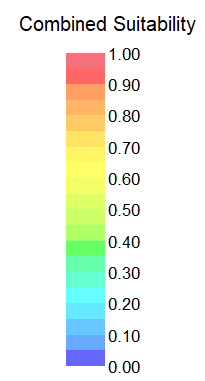
\includegraphics[width=0.3\textwidth,valign=t]{images/suitability_index}}& 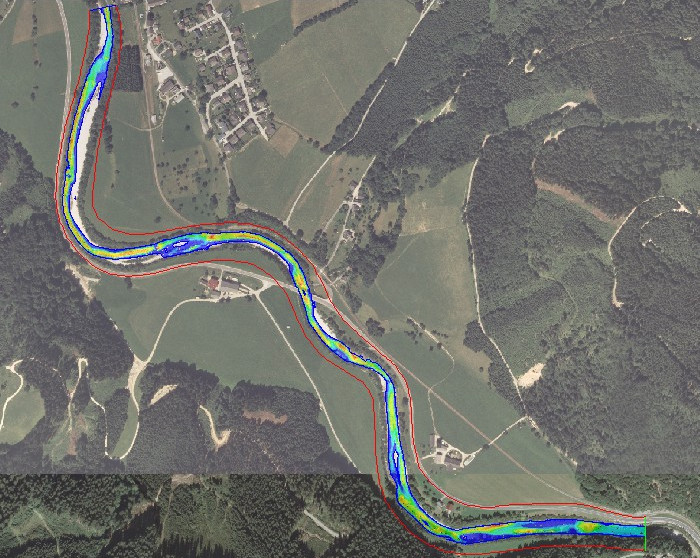
\includegraphics[width=0.56\textwidth,valign=t]{images/1_0216}\\
		& 1+ age class\\
		& 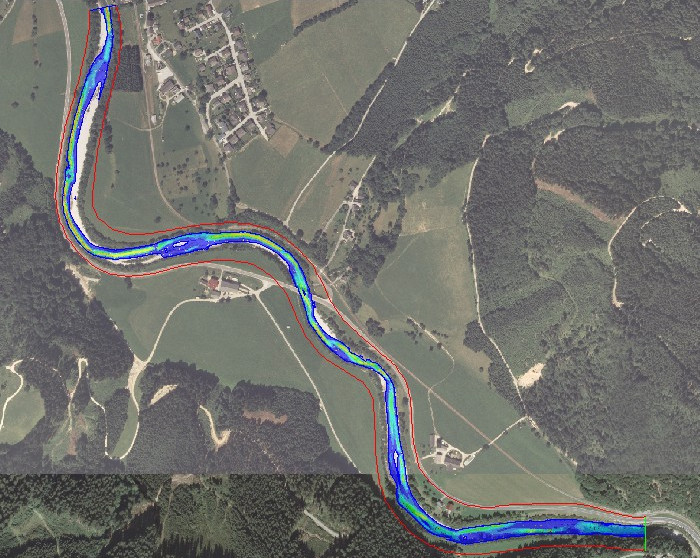
\includegraphics[width=0.56\textwidth,valign=t]{images/2_0216}\\
		& 2+ age class
		
	\end{tabular}
	\label{fig:0216}
	
	\caption{River2d models of the Ybbs river at \SI[per-mode=symbol]{2.16}{\cubic\meter\per\second}.}   %% figure Caption
	
\end{figure}


\newpage                                                                %% End page


%%----------------Appendix C
\fakesubsection{\SI[per-mode=symbol]{6}{\cubic\meter\per\second} flow rate models} %% Adds subsection to TOC but not the page
\subsection*{Appendix C}\label{appendixC}                        %% Adds subsection to page but not the TOC

\renewcommand\thefigure{A.\arabic{figure}}                          %% Begins numbering the appendix figures with A
\setcounter{figure}{0}                                              %% Restarts the figure counter

\centering
\begin{figure}[h!]                                                   	%% 00.35 Flow rate
	\begin{tabular}{ l  c }
		
		& 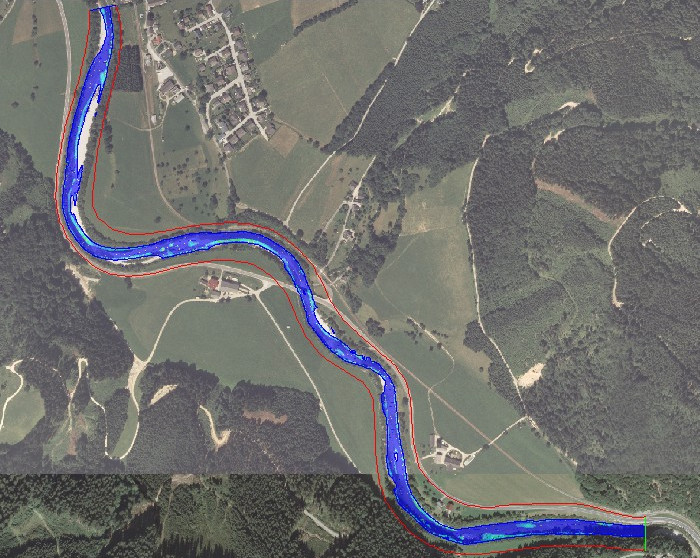
\includegraphics[width=0.56\textwidth,valign=t]{images/0_0600}\\
		& 0+ age class\\
		\multirow{4}{*}{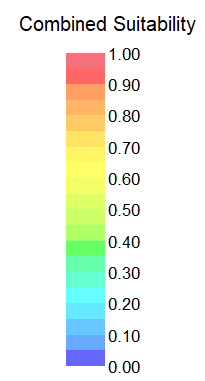
\includegraphics[width=0.3\textwidth,valign=t]{images/suitability_index}}& 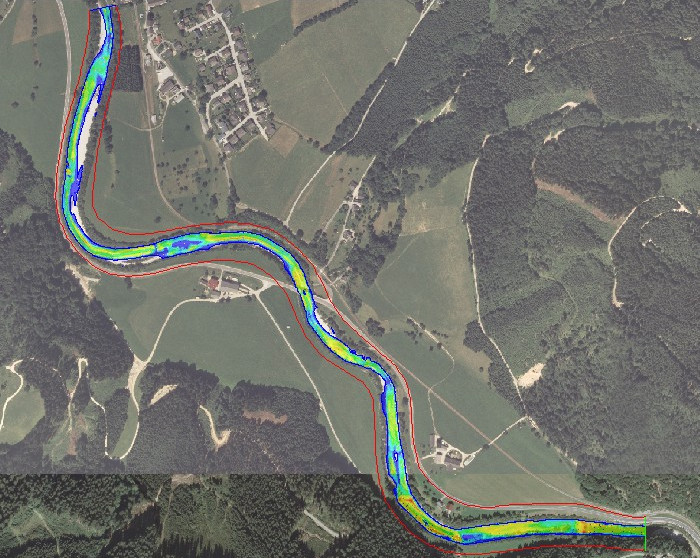
\includegraphics[width=0.56\textwidth,valign=t]{images/1_0600}\\
		& 1+ age class\\
		& 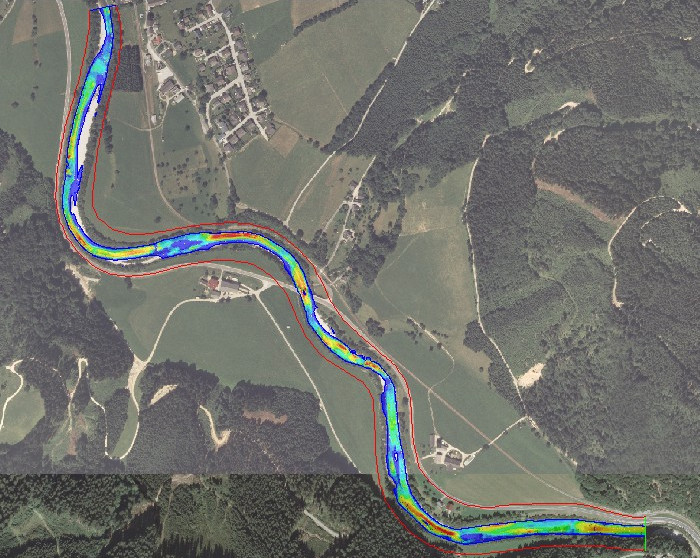
\includegraphics[width=0.56\textwidth,valign=t]{images/2_0600}\\
		& 2+ age class
		
	\end{tabular}
	\label{fig:0600}
	
	\caption{River2d models of the Ybbs river at \SI[per-mode=symbol]{6.00}{\cubic\meter\per\second}.}   %% figure Caption
	
\end{figure}


\newpage                                                                %% End page


%%----------------Appendix D
\fakesubsection{\SI[per-mode=symbol]{13}{\cubic\meter\per\second} flow rate models} %% Adds subsection to TOC but not the page
\subsection*{Appendix D}\label{appendixD}                        %% Adds subsection to page but not the TOC

\renewcommand\thefigure{A.\arabic{figure}}                          %% Begins numbering the appendix figures with A
\setcounter{figure}{0}                                              %% Restarts the figure counter

\centering
\begin{figure}[h!]                                                   	%% 00.35 Flow rate
	\begin{tabular}{ l  c }
		
		& 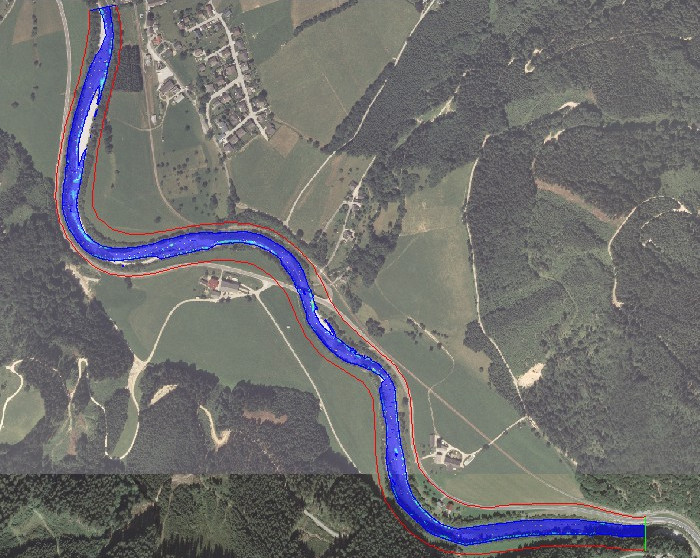
\includegraphics[width=0.56\textwidth,valign=t]{images/0_1300}\\
		& 0+ age class\\
		\multirow{4}{*}{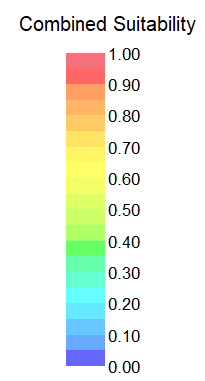
\includegraphics[width=0.3\textwidth,valign=t]{images/suitability_index}}& 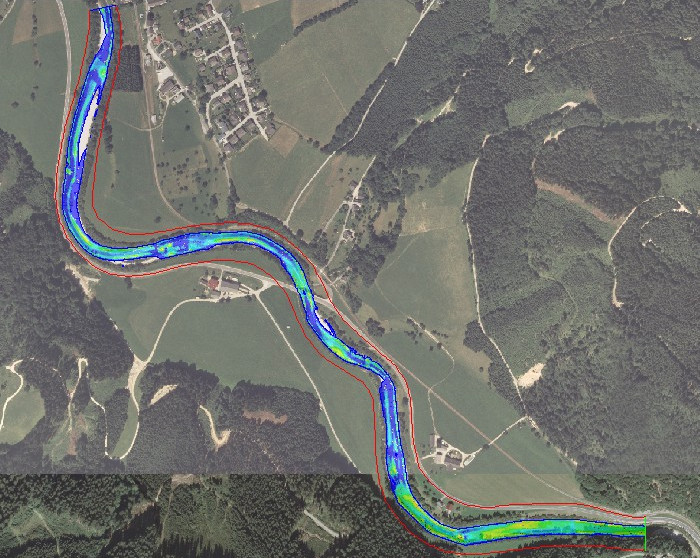
\includegraphics[width=0.56\textwidth,valign=t]{images/1_1300}\\
		& 1+ age class\\
		& 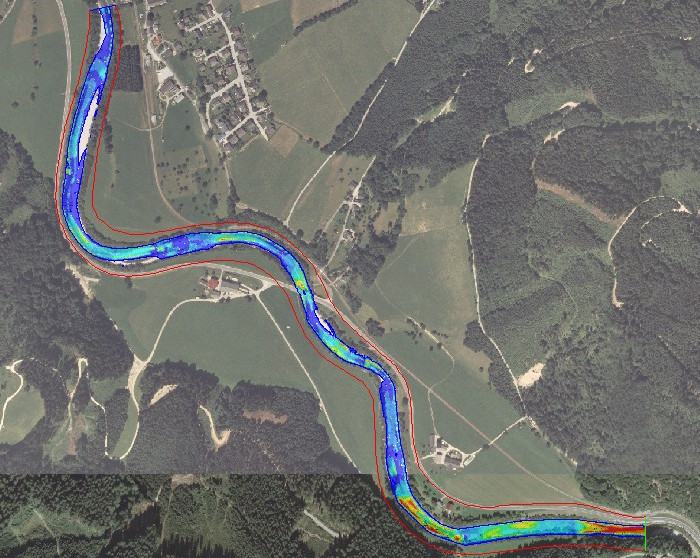
\includegraphics[width=0.56\textwidth,valign=t]{images/2_1300}\\
		& 2+ age class
		
	\end{tabular}
	\label{fig:1300}
	
	\caption{River2d models of the Ybbs river at \SI[per-mode=symbol]{13.00}{\cubic\meter\per\second}.}   %% figure Caption
	
\end{figure}


\newpage                                                                %% End page


%%----------------Appendix E
\fakesubsection{\SI[per-mode=symbol]{20}{\cubic\meter\per\second} flow rate models} %% Adds subsection to TOC but not the page
\subsection*{Appendix E}\label{appendixE}                        %% Adds subsection to page but not the TOC

\renewcommand\thefigure{A.\arabic{figure}}                          %% Begins numbering the appendix figures with A
\setcounter{figure}{0}                                              %% Restarts the figure counter

\centering
\begin{figure}[h!]                                                   	%% 00.35 Flow rate
	\begin{tabular}{ l  c }
		
		& 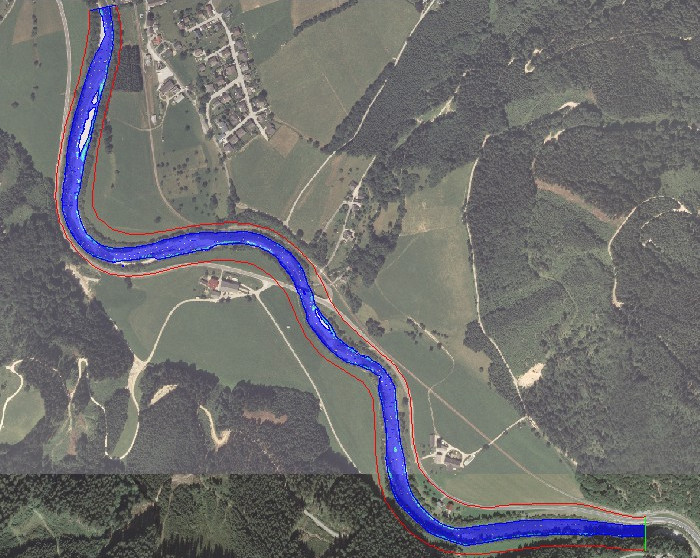
\includegraphics[width=0.56\textwidth,valign=t]{images/0_2000}\\
		& 0+ age class\\
		\multirow{4}{*}{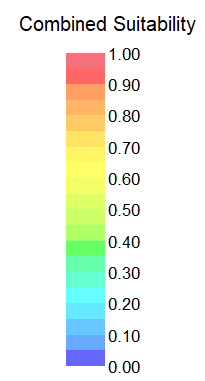
\includegraphics[width=0.3\textwidth,valign=t]{images/suitability_index}}& 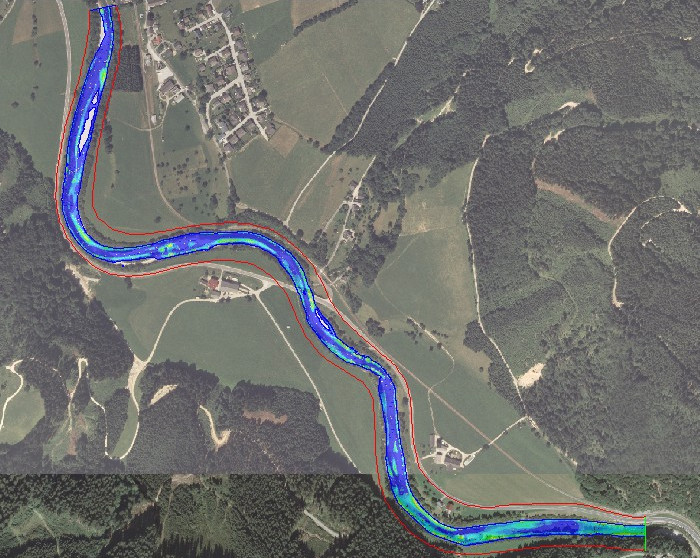
\includegraphics[width=0.56\textwidth,valign=t]{images/1_2000}\\
		& 1+ age class\\
		& 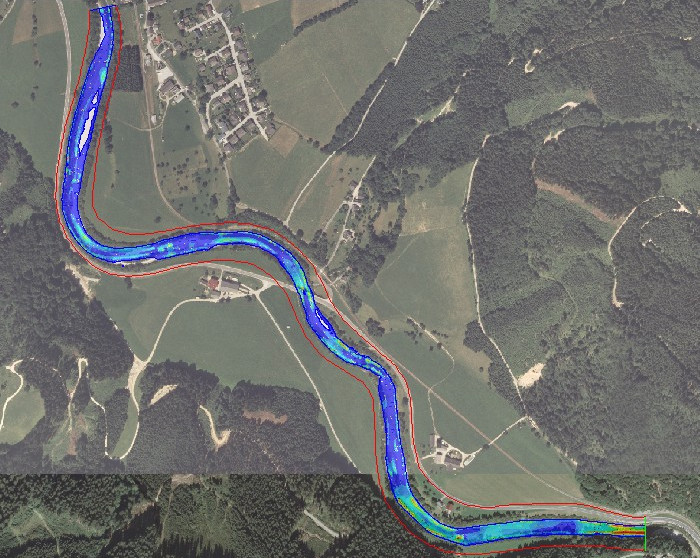
\includegraphics[width=0.56\textwidth,valign=t]{images/2_2000}\\
		& 2+ age class
		
	\end{tabular}
	\label{fig:2000}
	
	\caption{River2d models of the Ybbs river at \SI[per-mode=symbol]{20.00}{\cubic\meter\per\second}.}   %% figure Caption
	
\end{figure}


\newpage                                                                %% End page

